
We demonstrate how an awareness of skewness can allows us to define a QoI a-priori that will\---on average\---better resolve $\paramref$ by providing information in mutually distinct directions in $\pspace$.
We begin by revisiting the example in Section \ref{subsec:pde-example} involving the Poisson problem and uncertain boundary condition $g$.
Recall how $\qoi^\text{2D}$ was able to better resolve $\paramref$ than $\qoi^\text{1D}$.
The map $\qoi^\text{2D}$ was presented as an option for taking the same available hundred measurements and using them to form a more informative map.
In this chapter, we present a more detailed study of the construction of this map, reflecting a case-study in designing a problem where the QoI map is informative.

\section{Extension to Vector-Valued QoI Maps}
In our first example, we show that a small change in the decision of how to partition the measurements collected on the response surface can induce a 2-dimensional map $\qoi^\text{2D}_\prime$ which is ``effectively'' one-dimensional in that the two components provide highly correlated information.
Such a map is more skewed than the one we presented with $\qoi^\text{2D}$, and so leads to MUD-point solutions that exhibit similar behavior to those that we got when we used $\qoi^\text{1D}$ in the original problem.
This decreased precision demonstrates that skewness\---although developed in the previous chapter within the context of set-valued solutions\---is still a relevant measure of a map's utility when solving parameter identification problems.

The examples in Sections~\ref{subsec:ode-example} and \ref{subsec:pde-example} motivate the use of a data-constructed QoI in order to incorporate an arbitrary number of measurements in a system into a scalar-valued map.
These examples were chosen so that $\text{dim}({\Lambda}) = 1$ for simplicity and to establish a baseline for convergence results.
The linear examples in Section~\ref{sec:high-dim-linear-example} demonstrate that the DCI framework maintains the accuracy of least-squares while incorporating initial beliefs for higher-dimensional linear maps.
In those examples, we showed that our ability to resolve a true parameter improved as the gap between input dimension and operator row-rank shrunk.

The rank-deficiency of an operator can be attributed either to ill-conditioning of an operator $A:P\to P$, or when $P>D$ for a full-rank $A:P\to D$.
In scenarios where $S>P$ observations are available, we are motivated to somehow leverage the form of Eq.~\eqref{eq:qoi_WME} to construct a vector-valued version incorporating subsets of $S$ for each component.
For example, a system for which spatial measurements are available over time may motivate constructing a scalar-valued WME map for each spatial location.
If distinctly different observable quantities are available (ones perhaps with different physical units), then these may be collapsed into each component of the map.

The discussion of how to optimally construct such maps is beyond the scope of this work, and would need to take into account nuances involving measurement sensitivities and address combinatorial design-spaces.
However, we summarize that the extension of the equations presented in Section~\ref{sec:MUD_analysis} follows directly by constructing the resultant $1\times P$ matrices $A$ and scalar-valued $b$ for each component and then stacking them to form a $D\times P$ system, where we are motivated to minimize $P-D$.

%%%%%%%%%%%%%%%%%%%%%%%%%%%%%%%%%%%%%%%%%%%%%%%%%%%%%%%%%%%%%%%%%%%%
%%%%%%%%%%%%%%%%%%%%%%%%%%%%%%%%%%%%%%%%%%%%%%%%%%%%%%%%%%%%%%%%%%%%

% \subsection{A Vector-Valued QoI Map}
% In the PDE example of \ref{sec:pde-example}, we presumed knowledge about the structure of $g$ being a sine curve; we only had to estimate a scaling coefficient for it.
% To demonstrate the use of the WME QoI in solving inverse problems in higher dimensions, we set up the following series of examples in the same spirit with respect to the model and measurement locations, but presuming less about $g$ than before.
%
% We choose a polynomial function $g$ which exhibits similar behavior to the former sine curve, but without the symmetry about $x_2=0.5$, and scale it so that it takes a minimum at the same value as before (at $g = -3$).
% We selected $g(x) = \alpha x_2^2 (x_2 - 1)^5$, with $\alpha$ chosen to satisfy the aforementioned design specification (so that $g(x)=-3$ for $x=(0,\frac{2}{7})$).
% Suppose that as modelers, we are told only that $g$ is negative and bounded below by $-4$.
%
% We propose beginning to estimate it by placing two knots on the interior of the domain of $g$ and trying to deduce its value at these points.
% This gives us a parameter space of $\pspace = [-4, 0]$, and over this space we will assume a uniform density again.
% Our first two knots will be the equispaced points $x = (0,\frac{1}{3}), (0,\frac{2}{3})$, and the family of functions that this spans is visually illustrated in the left half of Figure~\ref{fig:pde-highd-initial-2d}.
% We also plot the true function and the associated piecewise--linear that comes from interpolating the true $g$.
% Observe that none of these (purple) functions we are considering to explain the data we collected (from the black curve) really adequately capture the correct dynamics, and that even the piecewise-linear interpolant (red) mis--characterizes the true boundary condition for most of the domain.
%
% The rest of the problem setup will be kept the same as the previous example, except that instead of $N=10,000$ parameter space samples, we use $N=1,000$.
% The reason for this is that we will not be doing the same convergence studies, so we are less interested in exhaustively exploring $\pspace$ than demonstrating that our method can handle a wider variety of inverse problems than the previous examples may suggest.


%
% \subsubsection{A Scalar-Valued QoI Map}
%
% Our first inverse problem involves solving the SIP with the same scalar-valued QoI map constructed by incorporating all the measurements into \eqref{eq:qoi_WME}.
% To give the reader a sense of the ability for this ``basis'' to match the one-hundred measurements used for inversion, we plot the best match of our thousand parameter samples with respect to these measurements in purple in the top half of Figure~\ref{fig:pde-highd-2d-projection}.
% There, we also plot the closest match to the interpolating piecewise-linear function in green, and note that we have a near-identical match among our thousand parameter samples, though the best predictor of the data we collected is a different sample.
% We are curious which of these two functions the MUD will more closely resemble.
% The residual Q-Q plots for the two functions are shown to illustrate the differences in misfit to provide an alternative view to the goodness-of-fit.
%
%
% \begin{figure}
% \centering
%   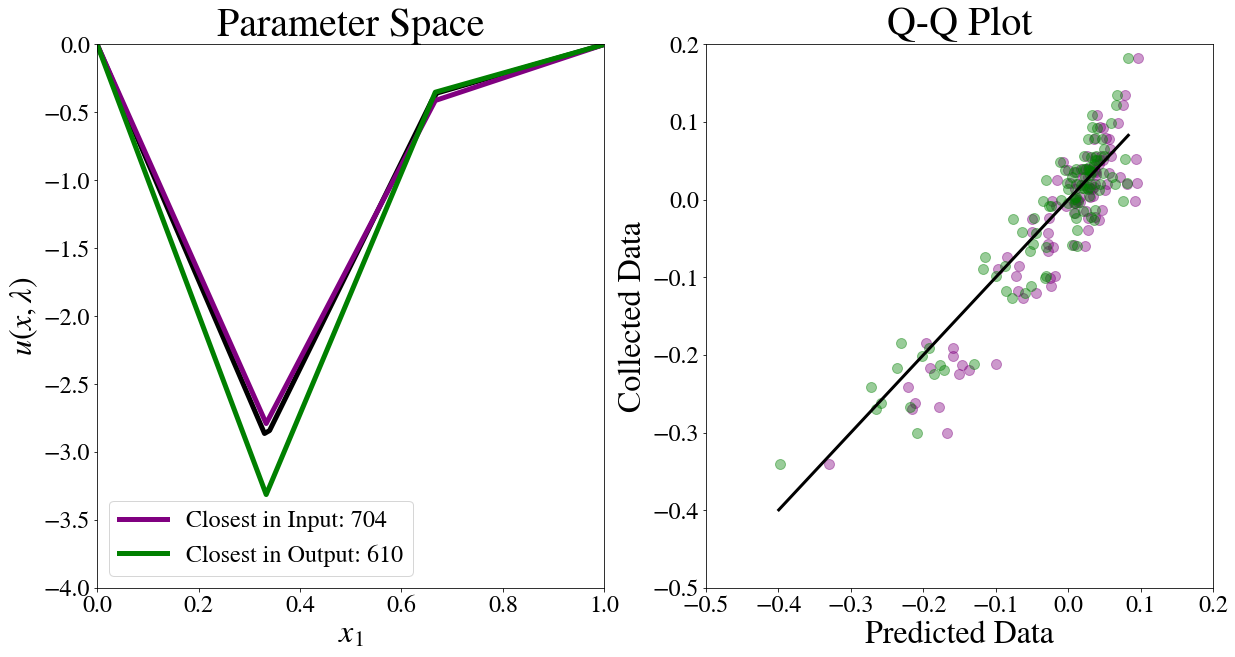
\includegraphics[width=0.95\linewidth]{figures/pde-highd/pde-highd_proj_D2.png}
% \caption{ TK - x-axis label needs to be fixed and this figure needs a proper caption.
% }
% \label{fig:pde-highd-2d-projection}
% \end{figure}
%
%
% In the bottom half of \ref{fig:pde-highd-2d-scalar-mud}, we show the MUD solutions arising from twenty trials using different observations of noise.
% Of particular interest is that the solutions seem to discover one of two types of explanations for the data, seemingly unable to decide which half of the domain represents a better estimate of $g$'s minimum value.
% As mentioned, this set of solutions comes from collapsing all hundred measurements into a scalar--valued QoI map, which negatively impacts our ability to identify the parameter in the problem, since our SIP is now $2\rightarrow 1$.
% [TK - cite Troy's result about dimensions from AWR paper] implies that we have an incentive to construct maps which ``close the gap,'' so to speak, between input and output dimension, to fully leverage the geometry of available information.
% The contour structure of the updated density samples plotted in red in \ref{fig:pde-highd-2d-example}.
%
% \begin{figure}
% \centering
%   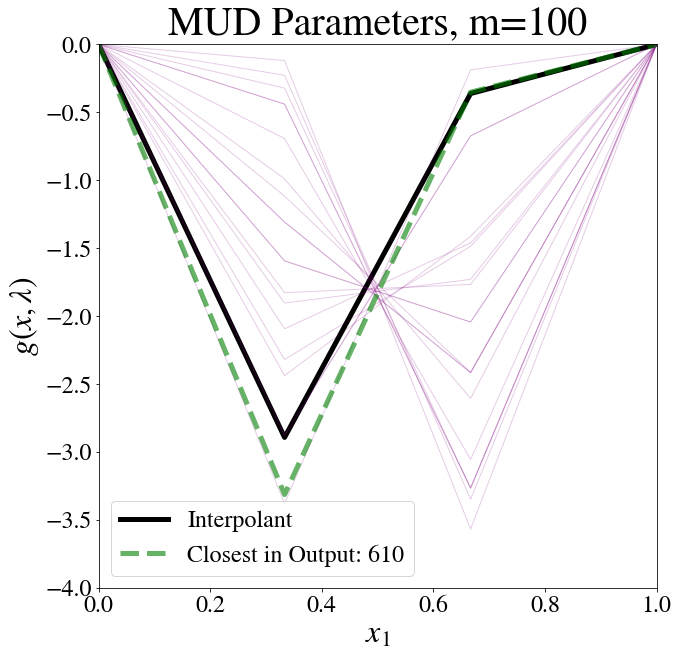
\includegraphics[width=0.95\linewidth]{figures/pde-highd/pde-highd_pair_D2-1_m100.png}
% \caption{ TK - x-axis label needs to be fixed and this figure needs a proper caption.
% }
% \label{fig:pde-highd-2d-scalar-mud}
% \end{figure}

\FloatBarrier
\subsection{Skewness and Vector-Valued QoI Maps}

Suppose that instead of constructing a scalar--valued QoI map, we used the form of \eqref{eq:qoi_WME} to construct a map with two components, yielding a $2 \rightarrow 2$ SIP instead.
We saw how such an approach could provide any tangible benefit for resolving the uncertainty in our true function $g$ in \ref{subsec:pde-example}, but presented the map $\qoi^\text{2D}$ without discussion of how it was selected.
To explore the impact of our choices in how $\Omega$ was partitioned into components of a QoI map, we propose two methods for splitting our hundred measurements into two subsets, which will be used to construct the respective components of the map according to \eqref{eq:qoi_WME}.
Both methods are shown in the top half of Figure~\ref{fig:pde-highd-2d-geometry}, and represent a bisection through $\Omega$ vertically to form $\qoi^\text{2D}_\prime$ and horizontally to form $\qoi^\text{2D}$.

\begin{figure}
\centering
  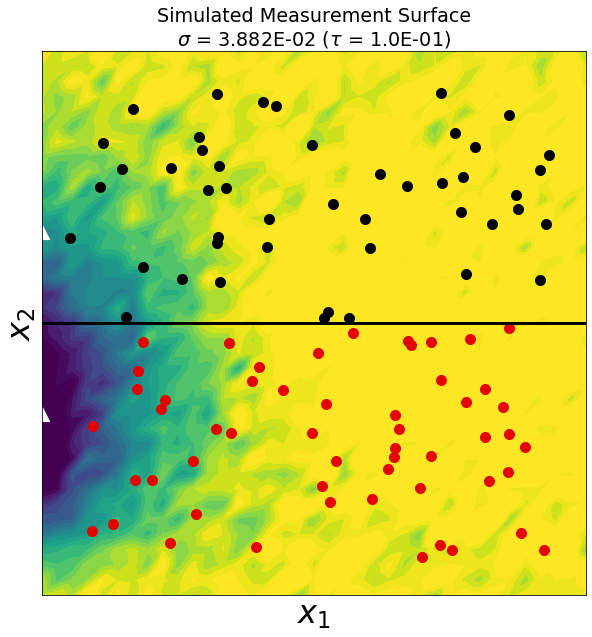
\includegraphics[width=0.475\linewidth]{figures/pde-highd/pde-highd_sensors_D2.png}
  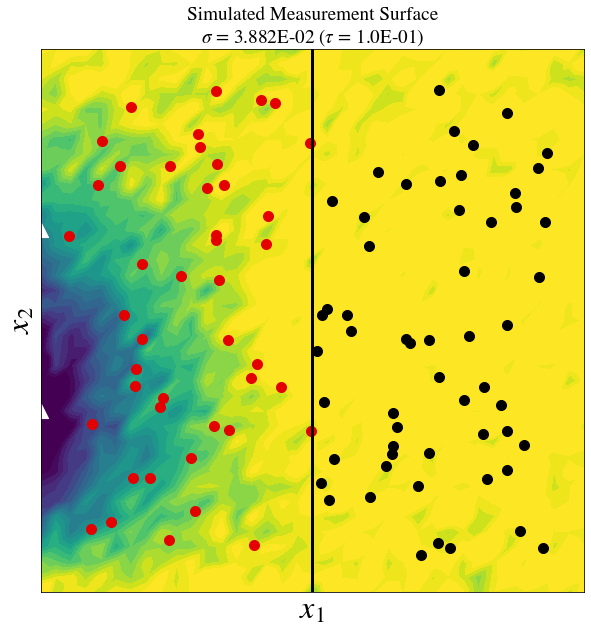
\includegraphics[width=0.475\linewidth]{figures/pde-highd/pde-highd_sensors-alt_D2.png}
  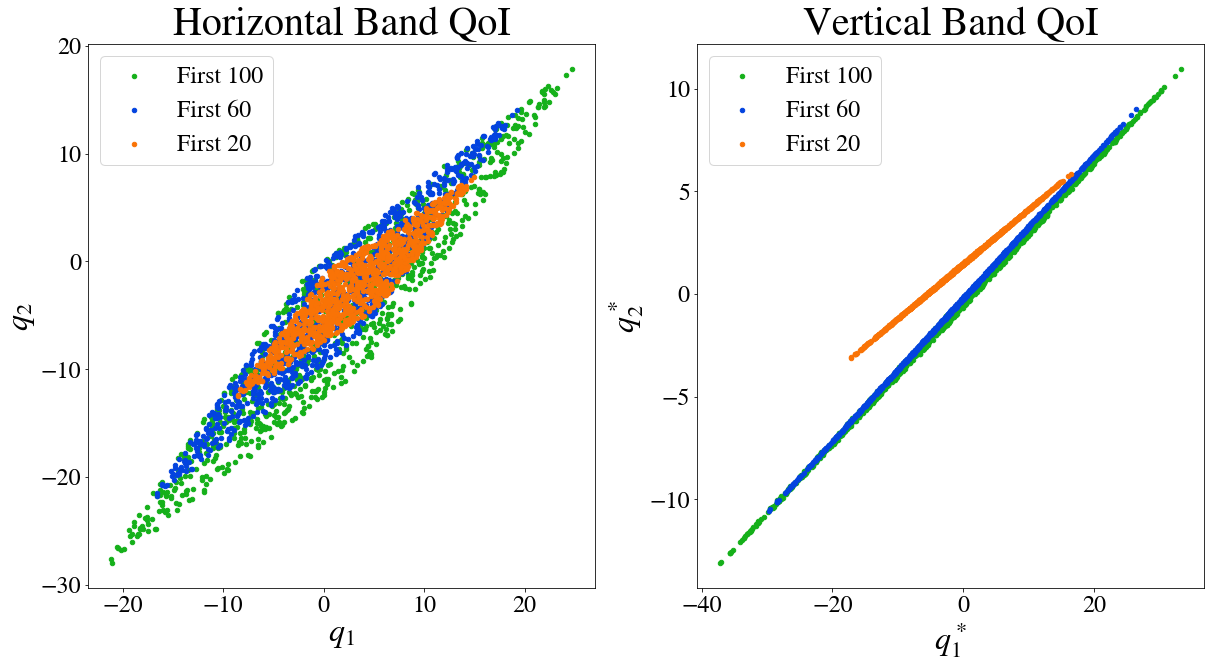
\includegraphics[width=0.95\linewidth]{figures/pde-highd/pde-highd_geom_D2.png}
\caption{
(Bottom): The vector-valued QoI map is constructed for all $N=10,000$ parameter evaluations and the two resulting vectors are plotted against one another for both methods of partitioning $\Omega$.
}
\label{fig:pde-highd-2d-geometry}
\end{figure}

We now highlight our approach to addressing the following question:
\begin{center}
\emph{With two QoI maps under consideration, which should we use?}
\end{center}

Before solving an inverse problem, there are a priori analyses that can be performed that can provide heuristics to help address these questions.
We first evaluate our thousand parameter samples through each of these maps and inspect the two-dimensional scatter-plots to build intuition about the underlying geometry induced by these maps.
We repeat this process for three subsets of the measurements (using the first samples in each half of $\Omega$ according to the random index assigned to them), and demonstrate the two resulting sets of relationship in the bottom half of Figure~\ref{fig:pde-highd-2d-geometry}.
This figure also shows the associated designs against the noisy response surface as a backdrop.

First, we note that the inclusion of more data points has the effect of dilating (and to some extent rotating) the induced data space for both QoI maps.
The geometric implication of this in the context of the chosen form of the QoI map has an interesting consequence.
Recall that the observed distribution remains a standard Gaussian, regardless of the number of data points used to construct the map.
In two dimensions, this observed distribution becomes a multivariate normal distribution instead, which can be visually thought of as a circular ``target'' located in the middle of each of the scatter-plots in Fig. \ref{fig:pde-highd-2d-geometry}.
As more measurements are incorporated, the size of that target relative to the rest of the space becomes increasingly small since the data manifolds dilate.
It is akin to finding the same needle in larger piles of hay.
More is asked of the solution to the SIP, since there are more measurements with which the model must agree.

The second implication of the two ways in which the maps can be formed is more visually evident, as the two quantities of interest that arise from a vertical bisection of $\Omega$ are nearly perfectly correlated.
In other words, $\qoi^\text{2D}_\prime$ has much higher skewness than $\qoi^\text{2D}$.
The two maps are presenting almost the same information (the shapes are very slim parallelograms), and so we fundamentally can already expect there to be very little difference between MUD points arising from using this map when compared to using the scalar--valued map.
Particularly since the observed distribution is radially symmetric, this problem\---while technically two-dimensional\---appears to be one-dimensional.

By contrast, the map induced by a horizontal split (bottom left of Fig. \ref{fig:pde-highd-2d-geometry}) provides new information in each component.
While there is some correlation (the manifolds are not rectangular), a far greater proportion of samples will fall within the practical support of the observed distribution, which qualifies them as possible solutions to the SIP.
More information is learned with the inclusion of each component using this design than would be with the vertical split.
Had we performed an analysis of average skewness, we could have discovered these geometric implications without visual inspection.
Using a quantitative measure such as skewness allows us to scale the assessment to higher-dimensional parameter space.

To this end, for the sake of brevity, we focus our attention on comparing the horizontal vector--valued QoI map to scalar ones (as proxies for highly-skewed maps), and note that a more fulfilling discussion of constructing QoI maps that induce desirable geometric properties is of interest for future work.
For the remainder of this example, the ``vector--valued'' map will refer to the the one which is split horizontally.
We note that this design, while not guaranteeing optimality for precision or accuracy's sake, at least respects the flow of information in the system being studied.
Since $\param$ is parameterizing the left Neumann boundary condition, information about its state flows from left to right in the horizontal direction.

\FloatBarrier
%%%%%%%%%%%%%%%%%%%%%%%%%%%%%%%%%%%%%%%%%%%%%%%%%%%%%%%%%%%%%%%%%%%%
%%%%%%%%%%%%%%%%%%%%%%%%%%%%%%%%%%%%%%%%%%%%%%%%%%%%%%%%%%%%%%%%%%%%
\section{Extension to Higher Dimensions}
We present a scenario to further underscore the value of considering geometry when constructing a QoI map for use in solving a SIP to perform parameter identification.
We show that when the dimension of $\pspace$ is higher, the benefit from maximizing the dimension of $\dspace$ is even more considerable than what we observed in the two-dimensional cases.
In the second example, we illustrate how we could use the solution to the SIP for the two-dimensional case from \ref{subsec:nonlinear-example} to better construct the problem we pose in five dimensions.
In particular, we show the effect that this refinement of a 5-D parameter space has on the estimated boundary--condition functions $\widehat{g}$ induced by the MUD solutions to the 5-D SIP.

Suppose that an experimenter less familiar with parameterization of curves and the problems associated with high-dimensions decided to start with a five--dimensional problem (five knots to describe $g$ instead of two), trying to accomplish greater granularity in the ability to estimate $g$, and imposes the same type of uniform initial density in each direction, yielding a parameter space of $\pspace = [-4, 0]^5$.
In Figure~\ref{fig:pde-highd-initial}, we show what such initial functions would look like, and note that many of them appear to exhibit fluctuating behavior for which the mesh ($36\times36$) being used to solve the problem, would not be fine enough to resolve.
This choice of initial density induces a lot of noise into the SIP we are hoping to solve, since ``common sense'' from a modeler's perspective could rule out zig-zag functions from wasting a model-evaluation budget, which we fix at the same $N=1000$ samples as in the previous 2-D problems.
We address one way these observations can be incorporated into posing a better SIP in the next example.
To establish a baseline for what we could expect the best possible representations in this peculiar choice of ``basis'' could be, we again find the closest match to the interpolating and to the noiselesss measurement data and plot them alongside residuals in Figure~\ref{fig:pde-5d-proj}.

\begin{figure}
\centering
  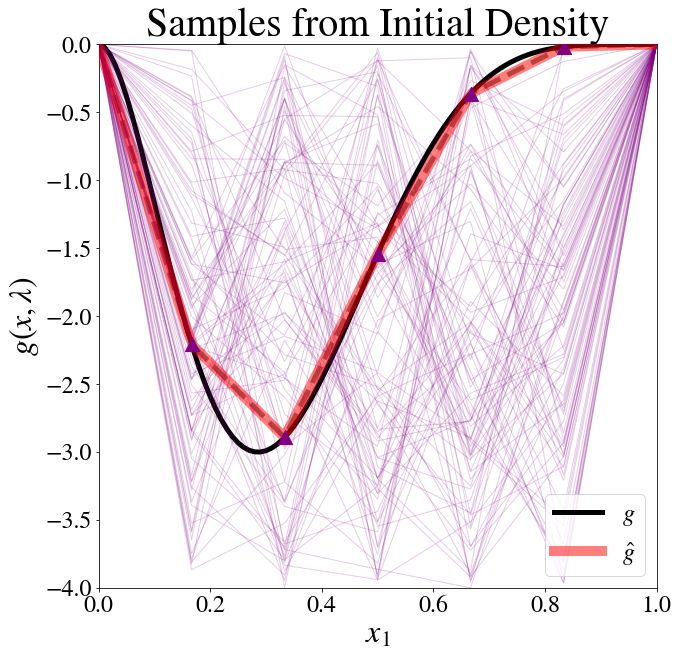
\includegraphics[width=0.475\linewidth]{figures/pde-highd/pde-highd_init_D5.png}
\caption{
One thousand initial parameter samples (our model evaluation ``bugdet'') were used to estimate $g$, constructed by taking independent uniform samples from $[-4, 0]$ for each direction are shown in purple.
}
\label{fig:pde-highd-initial-5d}
\end{figure}


\begin{figure}[htbp]
\centering
  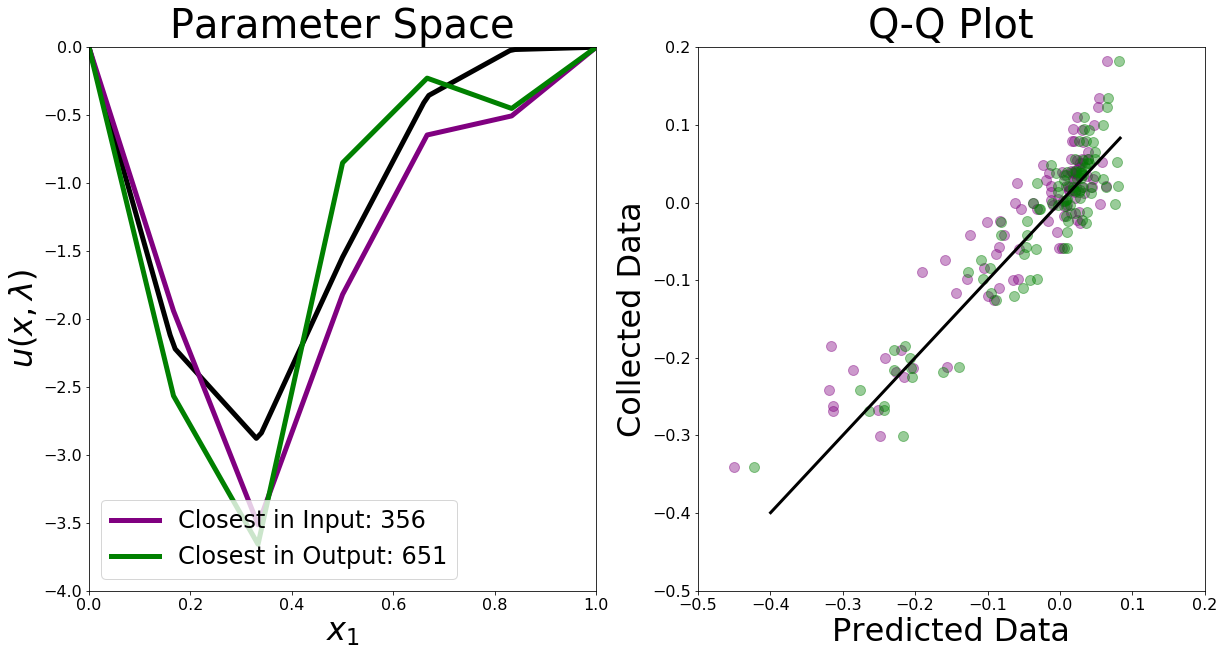
\includegraphics[width=0.675\linewidth]{figures/pde-highd/pde-highd_proj_D5}
\caption{
}
\label{fig:pde-5d-proj}
\end{figure}

Observe that in Figure~\ref{fig:pde-5d-proj}, both the closest fit in parameter and measurement space fail to resolve the true function behavior at $\lambda_5$ (the interpolating piecewise--linear is shown again for reference), and both place a minimum at $\lambda_2$.
The lines here are in some sense, the best that can be solved for with this design, and is helpful for comparing against our MUD solutions.
Of particular interest is that both functions under-estimate $g$ at $\lambda_2$ by a large margin.
Nevertheless, we pursue the solution for demonstration purposes and solve the SIP for both scalar-- and vector--valued QoI maps, the latter constructed with horizontal bands shown in the bottom left of Figure \ref{fig:pde-highd-5d-example}.

\begin{figure}[htbp]
\centering
  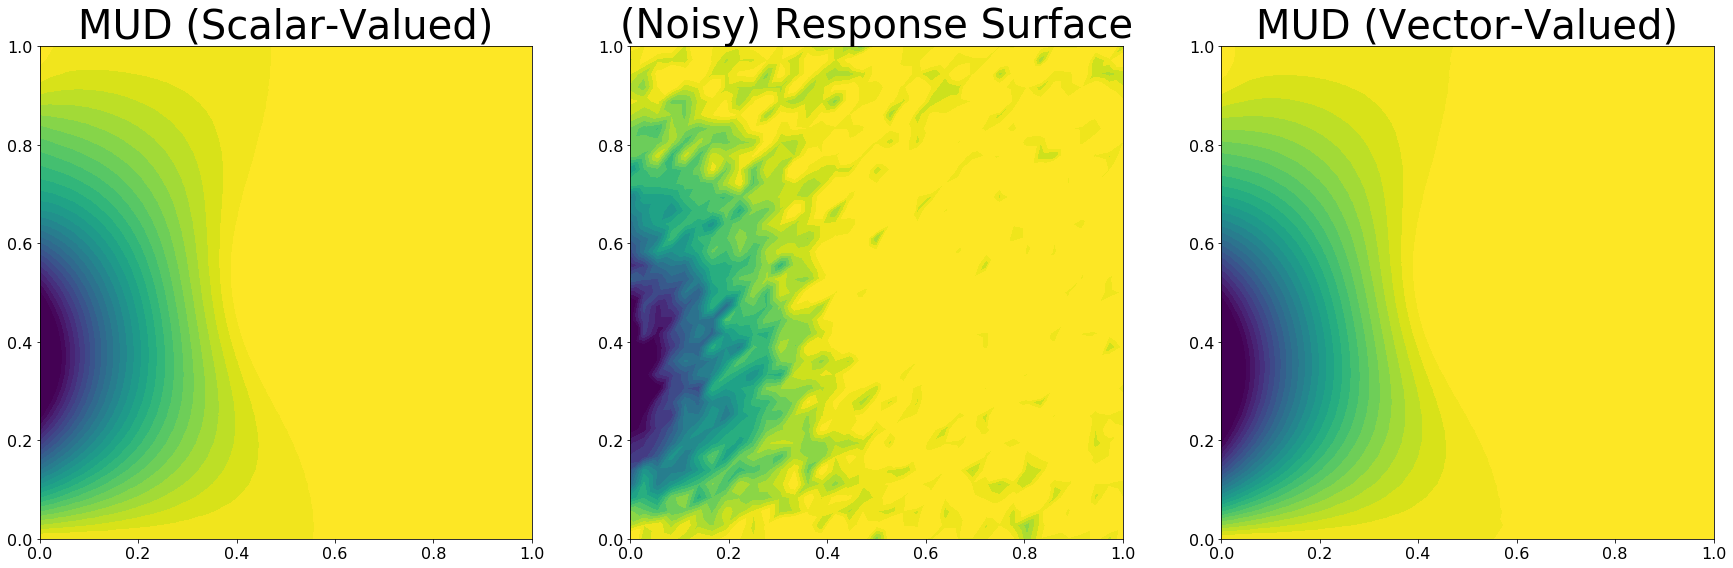
\includegraphics[width=0.95\linewidth]{figures/pde-highd/pde-highd_surf_exmud_D5_m100}
  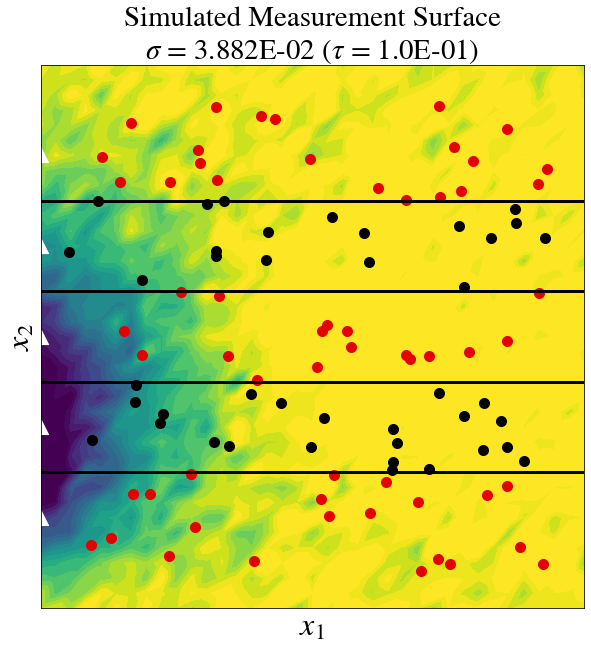
\includegraphics[width=0.35\linewidth]{figures/pde-highd/pde-highd_sensors_D5}
  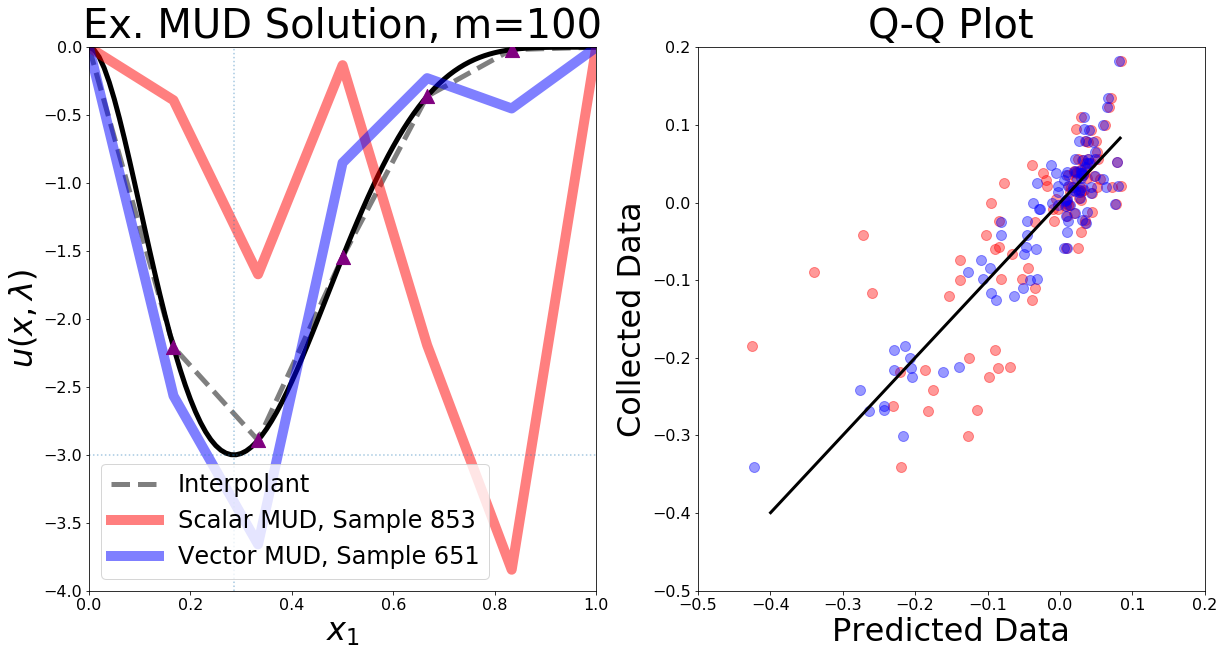
\includegraphics[width=0.6\linewidth]{figures/pde-highd/pde-highd_comp_exmud_D5_m100}
\caption{
(Top): Layout for 5-D vector--valued map and comparison of the two MUD solutions in parameter space.
(Bottom): The response surfaces predicted by the two QoI maps alongside the noisy response surface that generated the simulated collected data.
}
\label{fig:pde-highd-5d-example}
\end{figure}

In Figure~\ref{fig:pde-highd-5d-example}, the scalar-- and vector--valued MUD solutions are shown for the noisy surface plotted in the top-center, with associated predicted response surfaces flanking it.
In the bottom-center plot, we can see that the scalar-valued MUD completely misidentifies the location of $g$'s minimum value, but the vector-valued QoI is able to resolve the behavior much better.
In Figure~\ref{fig:pde-highd-5d-mud} we plot the results from twenty repeated trials (perturbations of noise) when using all hundred measurements, and observe the same difference in going from scalar-- to vector--valued solutions for the five--dimensional example that we saw in two dimensions with \ref{fig:pde-highd-2d-scalar-mud}\footnote{See Appendix (???) for examples of the twenty MUD-solutions using different numbers of measurements.}

\begin{figure}[htbp]
\centering
  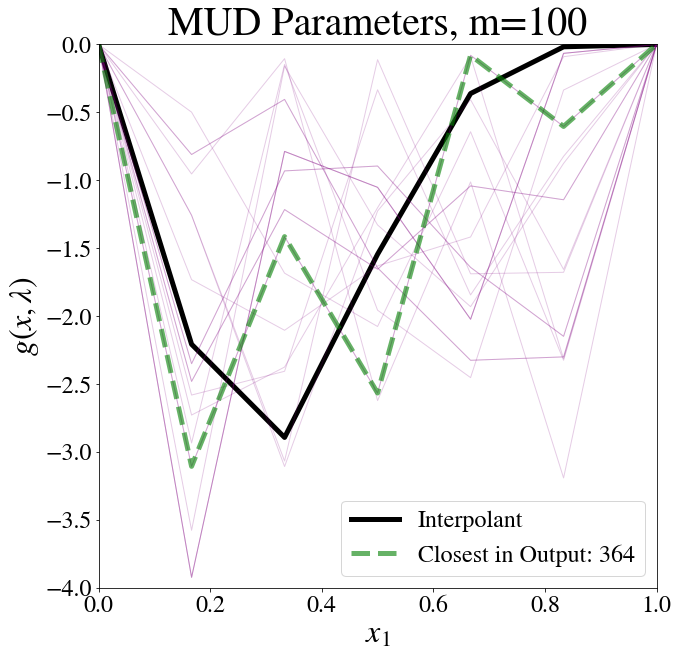
\includegraphics[width=0.95\linewidth]{figures/pde-highd/pde-highd_pair_D5-1_m100}
  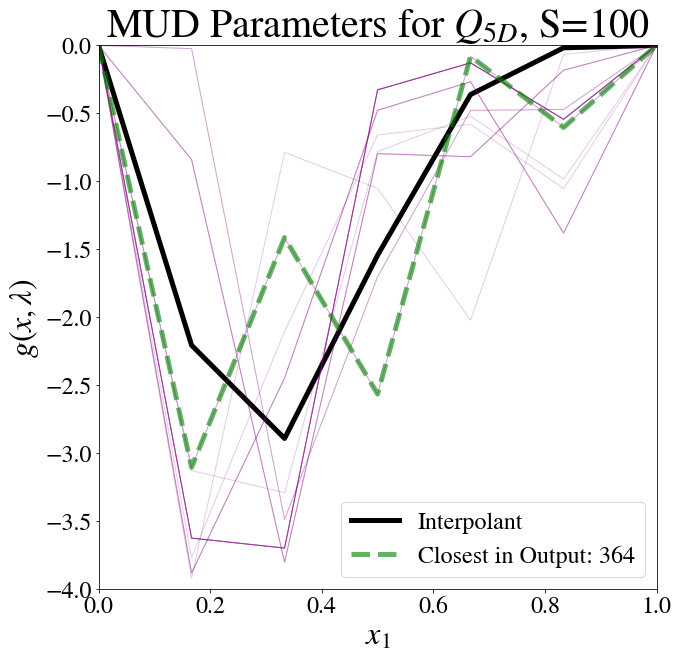
\includegraphics[width=0.95\linewidth]{figures/pde-highd/pde-highd_pair_D5-5_m100}
\caption{
(Top): Scalar-valued solutions.
(Bottom): Vector-valued solutions.
}
\label{fig:pde-highd-5d-mud}
\end{figure}

By increasing the number of quantities of interest used, more directions of uncertainty are resolved in the parameter space.
Since any solution in the equivalence class is valid for the SIP, the scalar-valued solutions are significantly more sensitive to noise, and so the solutions often appear to identify functions with a minimum on the wrong half of the spatial domain.
In the left half of Figure~\ref{fig:pde-highd-5d-mud}, the scalar-valued QoI is unable to differentiate between resolving residual discrepancies in different locations in $\Omega$.
By contrast, the vector-valued QoI shown below it is again constructed with respect to the flow of information in the system, and so many more of the twenty trials land closer to the true minimum value of $g$.
The solutions for the vector-valued approach instead explore the available knots (at $x_2=1/6$ and $1/3$), nearest the actual minimum value of $2/7$ instead, a much more valuable area of $\Lambda$ to explore.

Perhaps unsurprisingly given the poorly-designed initial density, our MUD solutions still do not really trace out the interpolants or projections from Fig~\ref{fig:pde-5d-proj} that we hope it should in order to approximate $g$.
At the very least, we would hope to accurately estimate the location and value of $g$'s minima.
Recall from \ref{subsec:nonlinear-example} that we previously solved a two-dimensional version of this problem, which could have been used to inform a much smaller region of two of the five directions to explore.
We now explore what would happen if our initial density was constructed with more care (without needing to use any model evaluations), since we saw from earlier examples that if DCI is initialized at a good initial mean, it has a chance of outperforming least-squares solutions in resolving discrepancy in truth.

%%%%%%%%%%%%%%%%%%%%%%%%%%%%%%%%%%%%%%%%%%%%%%%%%%%%%%%%%%%%%%%%%%%%
%%%%%%%%%%%%%%%%%%%%%%%%%%%%%%%%%%%%%%%%%%%%%%%%%%%%%%%%%%%%%%%%%%%%

\subsection{Alternative Experimental Approach}

As we proceed from two to five dimensions, being weary of the fact that we are fighting against the curse of dimensionality, we want to be more intelligent with our specification of an initial density.
Let us take a look at the samples that show up in black on the right of Figure~\ref{fig:pde-highd-2d-scatter} from a different perspective.
These represent samples from the updated density solved by incorporating all thousand measurements.
Instead of looking at high-probability samples as locations in $\pspace$, let us inspect them as a family of functions that are defined on the unit interval and use the envelope curves they sweep out to inform the specification of a better initial density; consider Figure~\ref{fig:pde-highd-5d-study}.

\begin{figure}[htbp]
\centering
  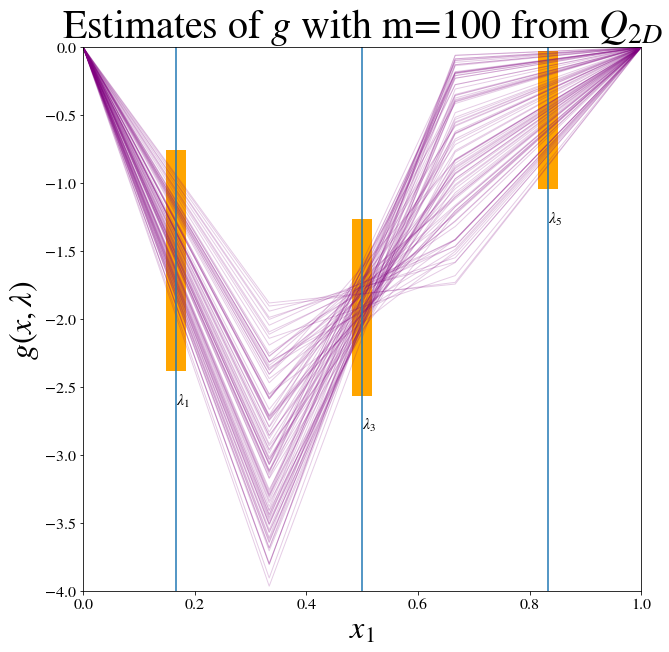
\includegraphics[width=0.675\linewidth]{figures/pde-highd/pde-highd-alt_initial_D5_m100.png}
\caption{
By considering the relationship between the parameters and the types of functions that could be possible given the solution to a 2-D inverse problem, we are able to create a more restricted parameter space in 5-D.
Knowledege of the behavior of $g$ at the boundaries allows for more than half of each of the three remaining intervals to be ruled out as infeasible regions when we look at high-probability samples from the 2-D SIP solution.
}
\label{fig:pde-highd-5d-study}
\end{figure}

The samples whose relative ratios exceeded $1/1000$ sweep out a family of curves that can be used to estimate bounds not only on $\lambda_2$ and $\lambda_4$ (the previous $\lambda_1$ and $\lambda_2$ from the 2-D problem)\---which exhibit correlation structure that we will turn to momentarily\---but also on the remaining three knots.
To form the intervals shown in orange in Fig.~\ref{fig:pde-highd-5d-study}, we take the upper and lower bounds of the curves passing through the vertical lines drawn at the three new knot values.
To be conservative, we multiply our lower bound by $1.2$ and the upper by $0.8$.
With these choices, we are still more than halving the interval-length in each direction as compared to the previous 5-D problem.
(Alternatively, one could establish a lower tolerance for accepting likely samples and avoid the multiplication factor, but a thorough exploration of how to best leverage the ratio of observed to predicted densities is left to future work.


\FloatBarrier
\subsubsection{A Better Initial Density}
For the two remaining directions, we want to capture the correlation structure that we were able to visually identify in Fig.~\ref{fig:pde-highd-2d-example} and impose something uniform-ish on it.
To achieve this, we perform a singular-value decomposition on the likely samples from the \emph{scalar}--valued 2-D solution, since there are so many more samples\footnote{ The scalar-valued contour was found to better characterize the direction of the equivalence class, suggesting perhaps a justifiable use for solving the problem with it. We could have formed an estimate of the updated density from using the vector--valued QoI and sampled from that instead. Many such approaches can be looked into in the future and are briefly discussed in the last section of this chapter.}.
The singular vectors are used to transform the vector-valued samples, and a uniform sampling is performed over the rectangular bounding box for these points, shown in the center of Figure~\ref{fig:pde-highd-2d-study}.
These generated samples, however, leave $\pspace$ when transformed back to their native space, as seen in the left panel.
To ameliorate this problem, we instead perform sampling in a while-loop, sampling from this uniform box and rejecting any that would get mapped back outside $\pspace$, until we reach our desired thousand samples.


\begin{figure}[htbp]
\centering
  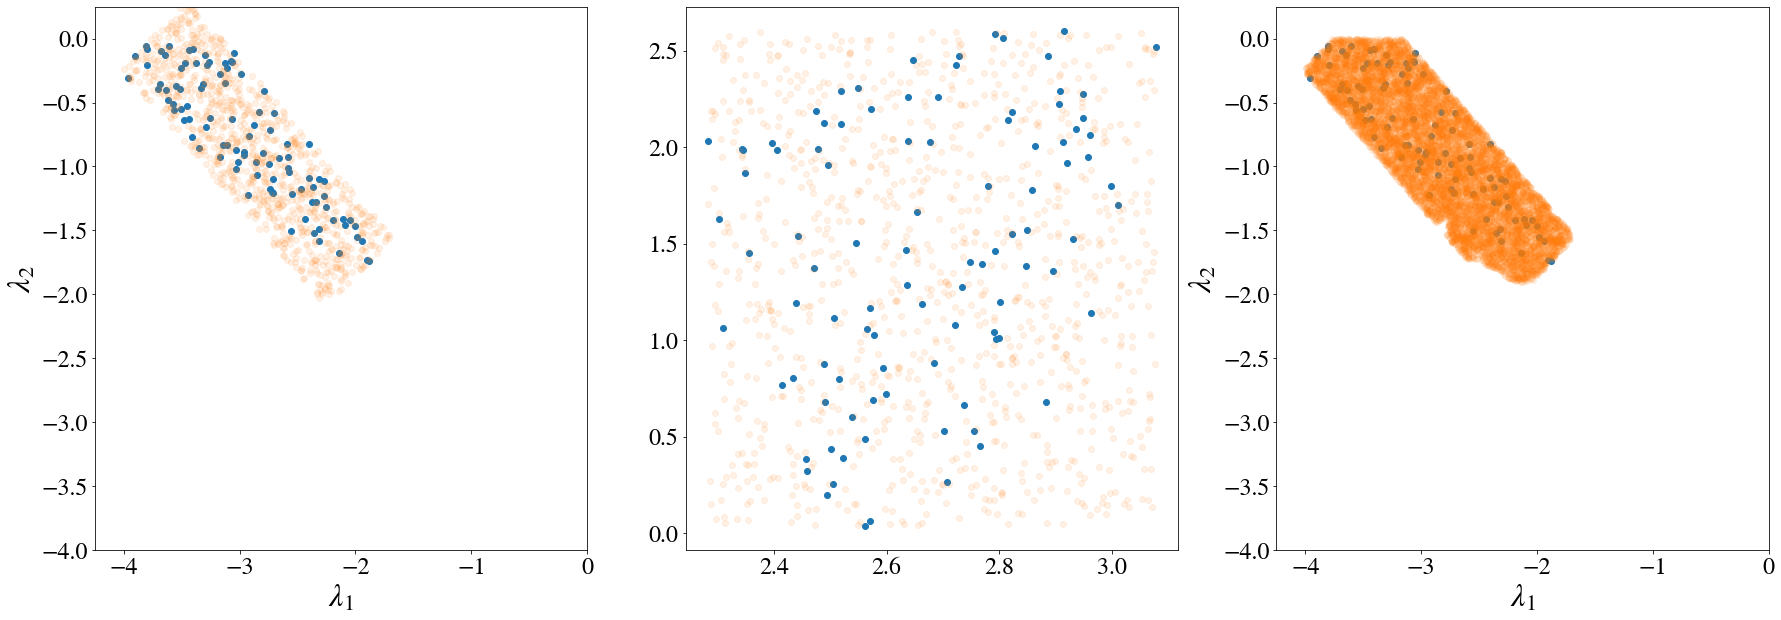
\includegraphics[width=0.95\linewidth]{figures/pde-highd/pde-highd-alt_initial_D2_m100}
\caption{
Generating proposal samples for the two directions informed by solving the 2-D inverse problem, aided by singular-value decompositions and an ad-hoc sampling procedure.
}
\label{fig:pde-highd-2d-study}
\end{figure}

Furthermore, note that in the center panel of Fig~\ref{fig:pde-highd-2d-study}, there are corner-regions of the space we want to avoid wasting samples on as well, so we reject samples that have squared two-norm greater than $0.05$ from their nearest vector--valued sample.
This sampling procedure produces the set shown in orange on the right side of the figure (ten thousand shown to demonstrate coverage).
We set out to define a computational analogue to an open cover for the relatively high-probability samples.
We keep one thousand of these 2-D samples, and join them with the three independent uniform sample sets of the same size taken from the intervals shown in Fig.~\ref{fig:pde-highd-5d-study} to form our new initial sample set, the functions from which generate the curves shown in Figure~\ref{fig:pde-highd-alt-initial-5d}.

\begin{figure}[htbp]
\centering
  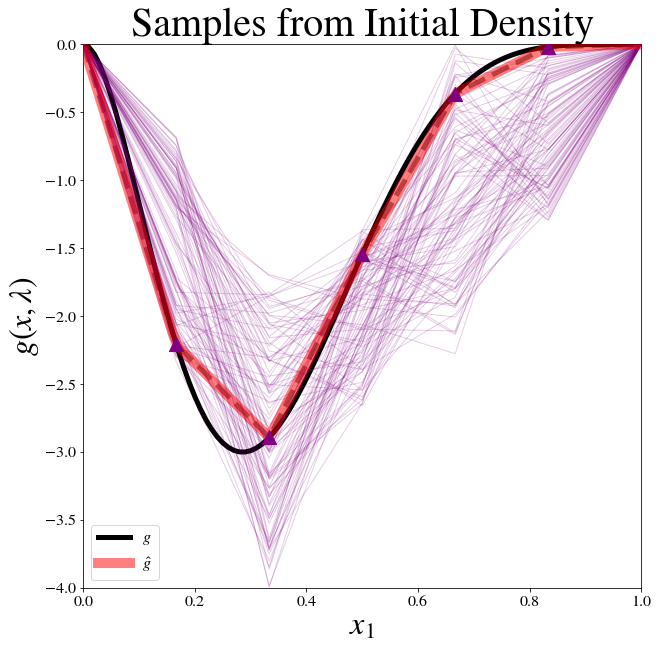
\includegraphics[width=0.675\linewidth]{figures/pde-highd/pde-highd_init_D5-alt}
\caption{
Initial density constructed for the second attempt at the five--dimensional inverse problem, with the structure of solutions learned from the 2-D example incorporated into the selection of bounds in each direction.
}
\label{fig:pde-highd-alt-initial-5d}
\end{figure}

The new initial curves in \ref{fig:pde-highd-alt-initial-5d}\---especially when contrasted to those in Fig.~\ref{fig:pde-highd-initial-5d}\---represent a far more reasonable set of possibilities.
The slope of the functions considered now all only have a single sign change, a marked improvement over the two or three that many samples from \ref{fig:pde-highd-initial-5d} exhibited.
We note that such considerations of smoothness could be avoided by parameterizing $g$ with a basis of some sort, but that problem is beyond the scope of this work.
Another possible improvement would be to incorporate the correlation structure that is present in the three other directions, derivable from a similar SVD-based analysis of the interpolation of the 2-D predictions through the new knot locations.
However, doing so would require more visual exploration than the authors deem worthwhile to demonstrate the point they are trying to make, which is that better initial densities improve the quality of solutions.

\begin{figure}[htbp]
\centering
  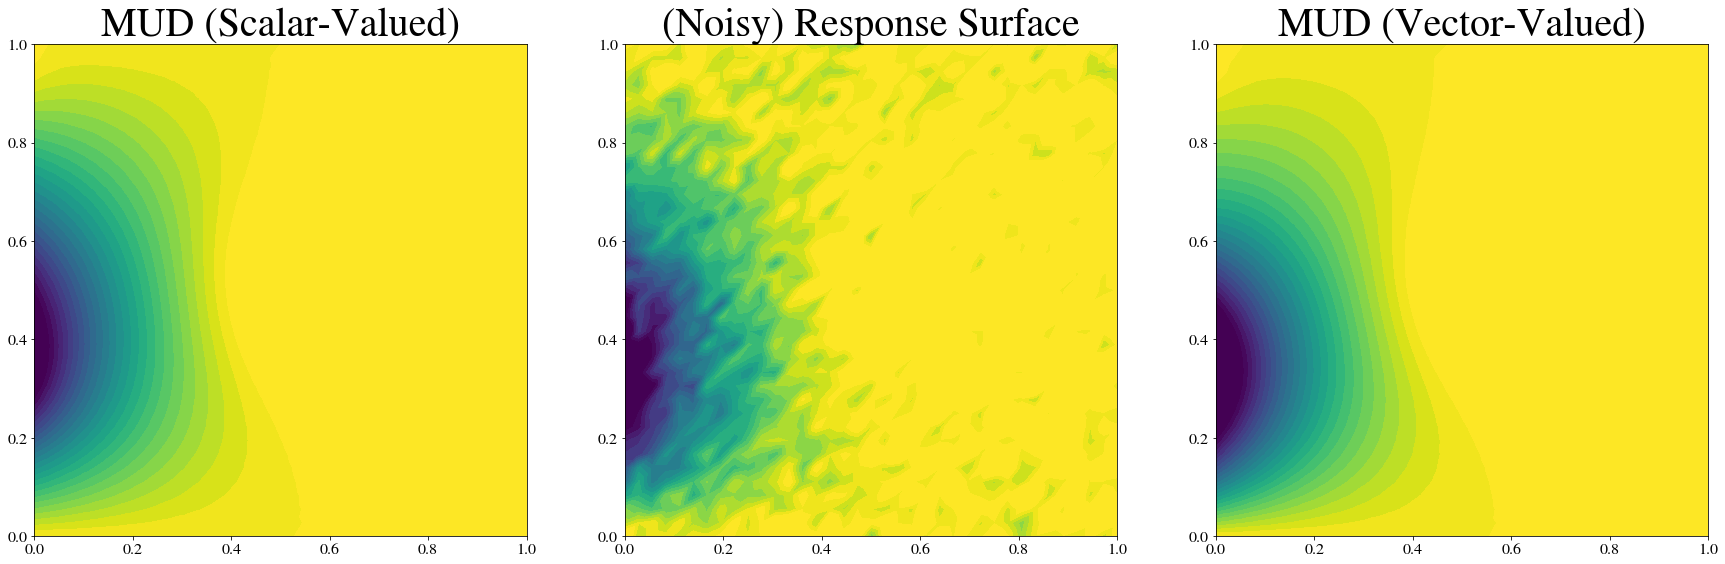
\includegraphics[width=0.95\linewidth]{figures/pde-highd/pde-highd_surf_exmud_D5-alt_m100.png}
  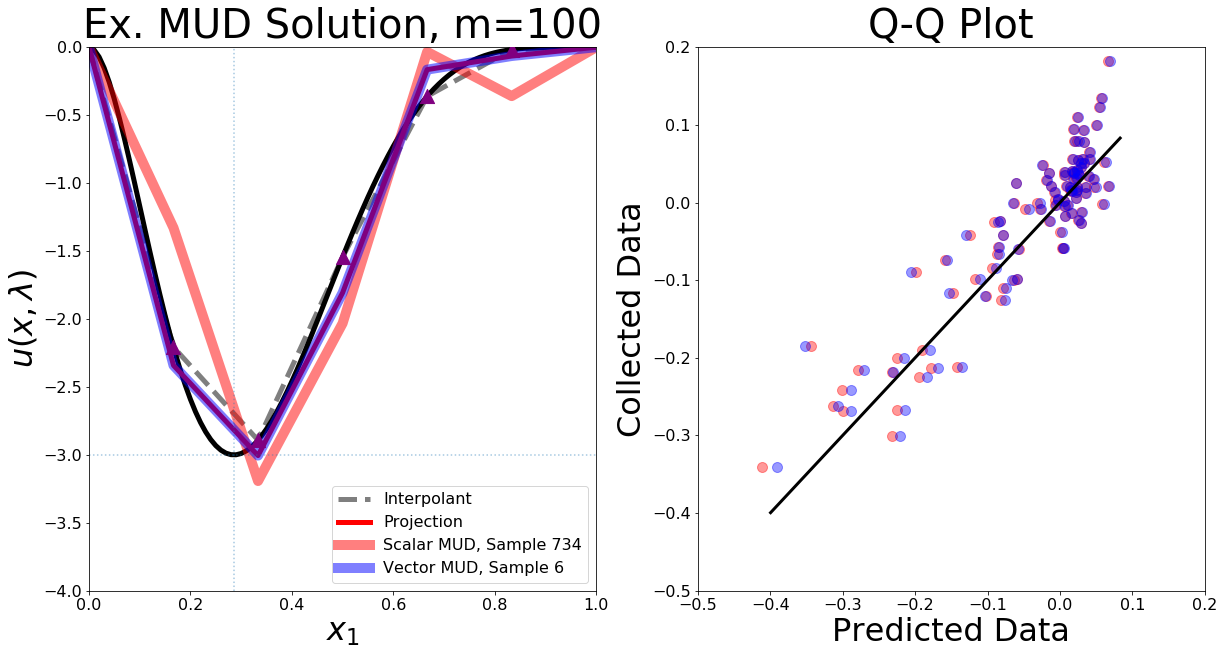
\includegraphics[width=0.9\linewidth]{figures/pde-highd/pde-highd-alt_comp_exmud_D5_m100.png}
\caption{
100 measurements for the revised five--dimensional problem yield substantially better estimates in the eyeball norm.
}
\label{fig:pde-highd-5d-alt-example}
\end{figure}


\subsection{Moving to Five Dimensions with more caution}

We now come to the solutions that arise from solving the same five--dimensional inverse problem of interpolating the values of $g$ through equispaced knot points, with both types of maps, in Figure~\ref{fig:pde-highd-5d-alt-mud}.
The difference in comparison to the example solutions in Fig.~\ref{fig:pde-highd-5d-mud} is stark: no longer are the solutions dramatically under-estimating the local minimum of $g$.
To the extent to which they fail to adequately to do is due to the insufficient resolution of five knot points; both scalar-- and vector--valued solutions identify the same knot as being the likely minimum, and the latter solution estimates the minima well (horizontal line drawn for reference) in the bottom-right plot.

Once again, we repeat the experiment twenty times to better understand the differences in the solutions relative to possible noise that polluted our measurements.
We are able to notice some interesting patterns by looking at the curves on the left side of Figure~\ref{fig:pde-highd-5d-alt-mud}.
First, we note that going from scalar-- to vector--valued resolves a significant amount of uncertainty in $\lambda_2$, $\lambda_3$, and $\lambda_4$.
Namely the QoI map appears to stop considering curves which do not have a sufficiently low minimum value.
Second, while the vector--valued MUD solution curves appear to capture the general characteristics of $g$ well, a number of them under-estimated the value at $\lambda_5$ quite severely relative to the true value (near zero), which we saw in Figure~\ref{fig:pde-highd-5d-mud} as well.

Even when only twenty measurements are incorporated into constructing the QoI maps, there is a considerable improvement in the predicted boundary conditions when using a better initial density, as seen by comparing the solutions in \ref{fig:pde-highd-5d-alt-mud-20} to \ref{fig:pde-highd-5d-mud-20} or \ref{fig:pde-highd-5d-mud}.

\begin{figure}[htbp]
\centering
  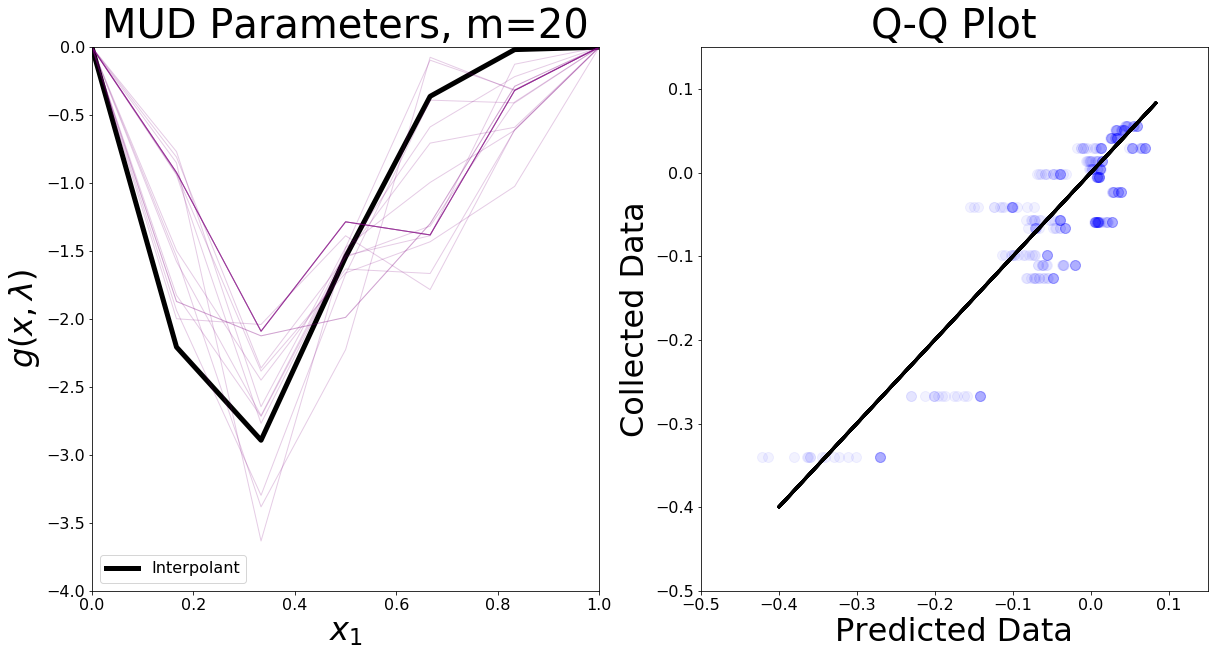
\includegraphics[width=0.95\linewidth]{figures/pde-highd/pde-highd_pair_D-alt-5-1_m20.png}
  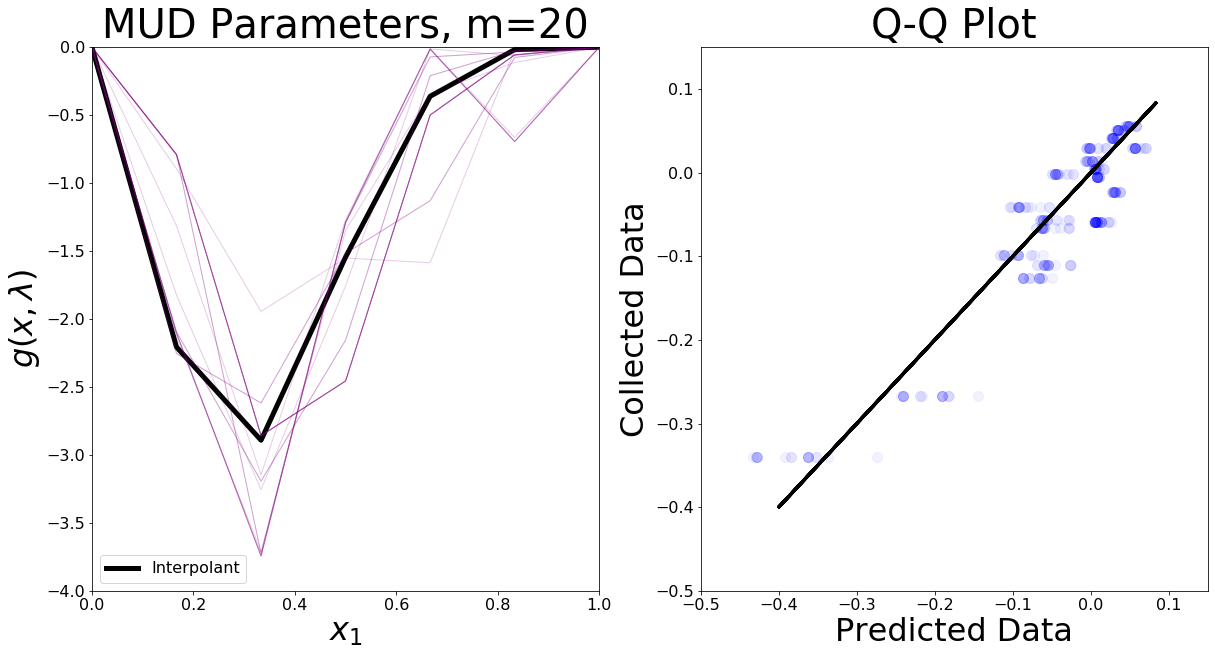
\includegraphics[width=0.95\linewidth]{figures/pde-highd/pde-highd_pair_D-alt-5-5_m20.png}
\caption{Solutions to the SIP using twenty measurements.
(Top): Scalar-valued solutions for alternative approach to the five-dimensional problem.
(Bottom): Vector-valued solutions.
}
\label{fig:pde-highd-5d-alt-mud-20}
\end{figure}

\begin{figure}[htbp]
\centering
  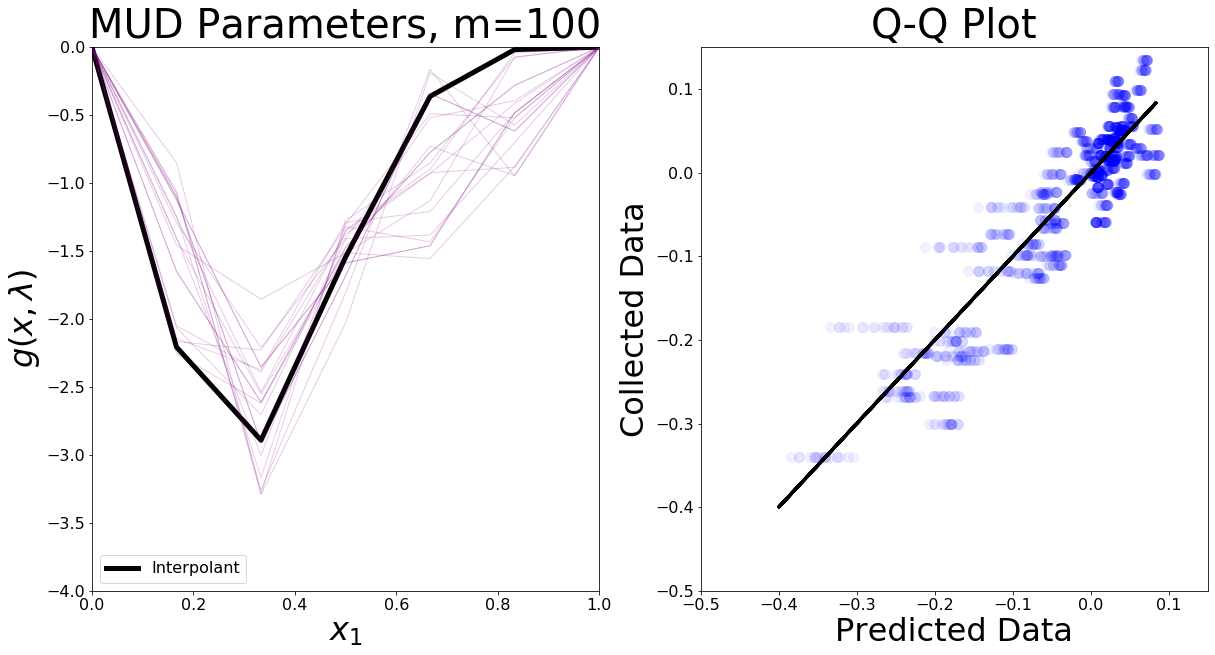
\includegraphics[width=0.95\linewidth]{figures/pde-highd/pde-highd_pair_D-alt-5-1_m100.png}
  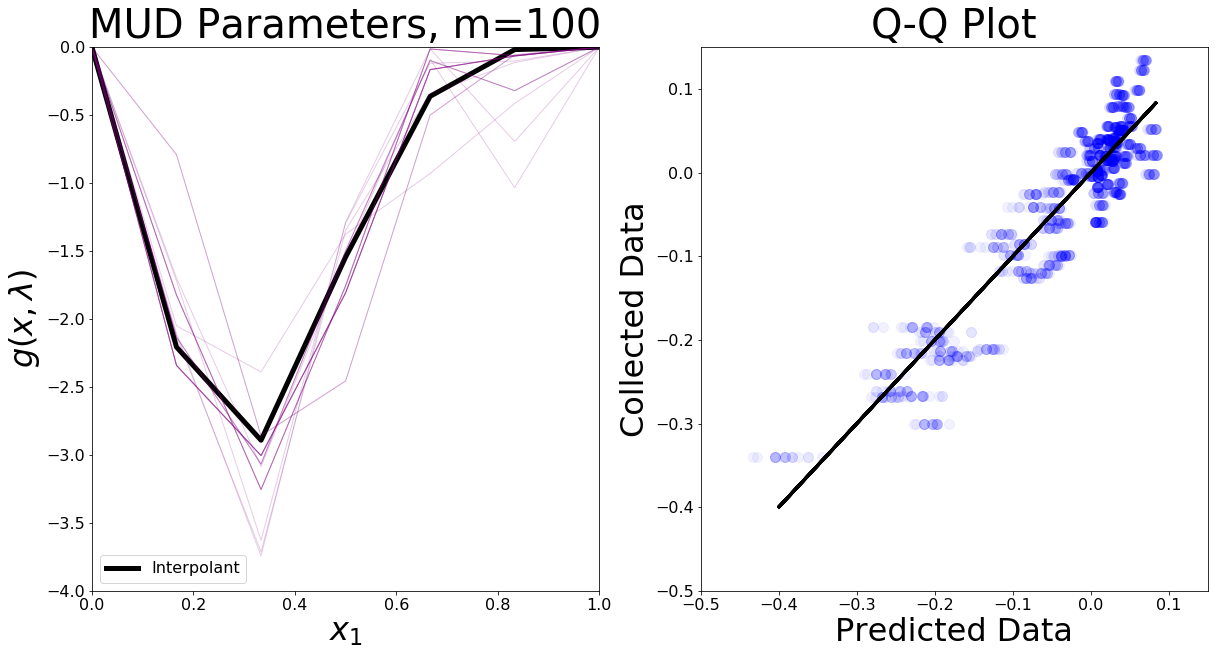
\includegraphics[width=0.95\linewidth]{figures/pde-highd/pde-highd_pair_D-alt-5-5_m100.png}
\caption{Solutions to the SIP using one hundred measurements.
(Top): Scalar-valued solutions for alternative approach to the five-dimensional problem.
(Bottom): Vector-valued solutions.
}
\label{fig:pde-highd-5d-alt-mud}
\end{figure}
\FloatBarrier

Because we began with a better choice of initial density, both QoI maps resolve the residuals similarly (bottom-left of \ref{fig:pde-highd-5d-mud}), and produce qualitatively similar estimates of the response surface. We attribute this to the fact that the vector--valued samples were used to bound the space, but note the direction was informed by the scalar--valued samples.

\subsubsection{Demonstration of Reduction in Uncertainty}

As a final note on this experiment, we contrast the resulting $L^2$-errors to $g$ \footnote{derived from computational approximation with the trapezoidal rule} of these MUD solutions, to the previous two examples in Figure~\ref{fig:pde-highd-5d-hist}, to show a lineage of learning, so to speak.
With each successive problem, our uncertainty is reduced and our MUD solutions lower in variance and increase in accuracy.
Note that they appear to be moving towards a value away from zero, which represents a fixed bias (five equispaced knots can only approximate this $g$ so well).

\begin{figure}[htbp]
\centering
  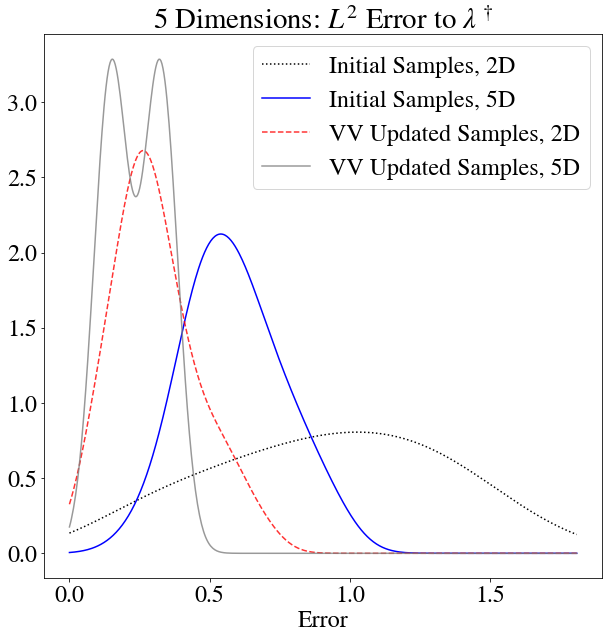
\includegraphics[width=0.675\linewidth]{figures/pde-highd/pde-highd_hist_D5_t5-0E-01}
\caption{
Comparison of the 2D initial errors to the 5D ones, as well as the reduction of uncertainty that solving a SIP problem for each provides.
}
\label{fig:pde-highd-5d-hist}
\end{figure}
